\documentclass[40pt,a4paper,UTF8]{ctexart}
\usepackage{amsmath}
\usepackage{graphicx}

\usepackage{float}

%输入带圈数字  eg:\textcircled{1}
\usepackage{fontspec,xunicode-addon}

%代码显示的包
\usepackage{listings}
\usepackage{xcolor}

%打出空心字母
\usepackage{amsfonts,amssymb}

%整体加粗
\usepackage{bm}

%公式按照章节标号
\numberwithin{equation}{section}

%长等号
\usepackage{extpfeil}

%注释用
\usepackage{comment}
%----------------------------------------------
%配置代码显示格式-掌握minted之前的替代品
%----------------------------------------------
\definecolor{codegreen}{rgb}{0,0.6,0}
\definecolor{codegray}{rgb}{0.5,0.5,0.5}
\definecolor{codepurple}{rgb}{0.58,0,0.82}
\definecolor{backcolour}{rgb}{0.95,0.95,0.92}

\lstdefinestyle{mystyle}{
	backgroundcolor=\color{backcolour},   
	commentstyle=\color{codegreen},
	keywordstyle=\color{magenta},
	numberstyle=\tiny\color{codegray},
	stringstyle=\color{codepurple},
	basicstyle=\ttfamily\footnotesize,
	breakatwhitespace=false,         
	breaklines=true,                 
	captionpos=b,                    
	keepspaces=true,                 
	numbers=left,                    
	numbersep=5pt,                  
	showspaces=false,                
	showstringspaces=false,
	showtabs=false,                  
	tabsize=2
}

\lstset{style=mystyle}



%-----------------------------------------------------------------------------------

\title{第六章作业}
\author{Student name: Francisrk}
\date{Due date: March 13th, 2022}

\begin{document}

\maketitle   %控制序列,能将在导言区中定义的标题、作者、日期按照预定的格式展现出来。

\section{第1题}
\paragraph{}
已阅。
\paragraph{}


\section{第2题}
\paragraph{}

\subsection{光流文献综述}
\begin{enumerate}
\item 按此文的分类,光流法可分为哪几类?


\item 在 compositional 中,为什么有时候需要做原始图像的 wrap?该 wrap 有何物理意义?


\item forward 和 inverse 有何差别?




\end{enumerate}


\subsection{forward-addtive Gauss-Newton 光流的实现}

\begin{enumerate}
\item 从最小二乘角度来看,每个像素的误差怎么定义?

参考\cite{ref2}定义原始图中每个点的像素为$I_1(x_i,y_i)$,第二张图中的每个点的像素为$I_2(x_i+\Delta x_i,y_i+\Delta y_i)$,则从最小二乘的角度来看,每个点的像素误差可以定义为:
\begin{align}
e_i=\underset{\Delta x_i,\Delta y_i}{min}||I_1(x_iy_i)-I_2(x_i+\Delta x_i,y_i+\Delta y_i)||_2^2
\end{align}


\item 误差相对于自变量的导数如何定义?

补充关于差分,微分和导数的区别\cite{ref1}
这里,待估计的变量是$\Delta x_i$和$\Delta y_i$,定义相应的导数为:
\begin{align}
\frac{\partial e_i}{\partial \Delta x_i}=-\frac{\partial I_2}{\partial \Delta x_i} \notag \\
\frac{\partial e_i}{\partial \Delta y_i}=-\frac{\partial I_2}{\partial \Delta y_i}
\end{align}
因为图像中每个点之间的像素值是离散的,不能直接用微分来求导,这里使用差分来代替微分来求导,使用中心差方式来进行求导计算。

令
\begin{align}
f(x+1,y)=I_2(x_i+\Delta x_i+1,y_i+\Delta y_i) \notag \\
f(x-1,y)=I_2(x_i+\Delta x_i-1,y_i+\Delta y_i) 
\end{align}
对其进行一阶泰勒展开:
\begin{align}
f(x+1,y)=f(x,y)+f'(x)  \notag \\
f(x-1,y)=f(x,y)-f'(x)
\end{align}
故对x有 
\begin{align}
f'(x)=\frac{f(x+1,y)-f(x-1,y)}{2}
\end{align}
对y有
\begin{align}
f'(y)=\frac{f(x,y+1)-f(x,y-1)}{2}
\end{align}

最终,相应的导数为:
\begin{align}
\frac{\partial e_i}{\partial \Delta x_i}=-\frac{\partial I_2}{\partial \Delta x_i}
=-\frac{I_2(x_i+\Delta x_i+1,y_i+\Delta y_i)-I_2(x_i+\Delta x_i-1,y_i+\Delta y_i)}{2}  \notag \\
\frac{\partial e_i}{\partial \Delta y_i}=-\frac{\partial I_2}{\partial \Delta y_i}
=-\frac{I_2(x_i+\Delta x_i,y_i+\Delta y_i+1)-I_2(x_i+\Delta x_i,y_i+\Delta y_i-1)}{2}
\end{align}
\end{enumerate}

\begin{lstlisting}[language=C++, caption=forward-addtive Gauss-Newton 光流的实现核心代码]
                    // TODO START YOUR CODE HERE (~8 lines)
                    //计算误差
                    double error = GetPixelValue(img1, kp.pt.x + x, kp.pt.y + y)-GetPixelValue(img2, kp.pt.x + x + dx, kp.pt.y + y + dy);
                    Eigen::Vector2d J;  // Jacobian
                    if (inverse == false)
                    {
                        // Forward Jacobian  前向雅可比(因为是离散的,不能用微分,使用中心差分方式来进行求导)
                        J = -1.0 * Eigen::Vector2d(
                                0.5 * (GetPixelValue(img2,kp.pt.x + dx + x + 1, kp.pt.y + dy + y)-GetPixelValue(img2, kp.pt.x + dx + x -1, kp.pt.y + dy + y)),
                                0.5 * (GetPixelValue(img2, kp.pt.x + dx + x, kp.pt.y+ dy + y + 1)- GetPixelValue(img2, kp.pt.x + dx + x, kp.pt.y + dy + y -1))
                                );
                    }
                    else
                    {
                        if(iter == 0 )
                        // Inverse Jacobian
                        // NOTE this J does not change when dx, dy is updated, so we can store it and only compute error
                        //反向模式,使用I1处的梯度替换I2处的梯度,雅可比不随dx,dy的改变而改变,所以不加dx,dy
                        {
                            J = -1.0 * Eigen::Vector2d(
                                    0.5 * (GetPixelValue(img2,kp.pt.x + x + 1, kp.pt.y + y)-
                                           GetPixelValue(img2, kp.pt.x +  x -1, kp.pt.y + y)),
                                    0.5 * (GetPixelValue(img2, kp.pt.x +  x, kp.pt.y + y + 1)-
                                           GetPixelValue(img2, kp.pt.x +  x, kp.pt.y + y -1))
                                    );
                        }
                    }
                    // compute H, b and set cost;
                    b += -error * J;
                    cost += error * error;
                    if(inverse==false || iter==0)  //如果是正向或者是第一次迭代,就需要更新系数矩阵H
                    {
                        H +=  J * J.transpose() ;  //这里的雅可比定义出来是J^T,直接就是向量,求H要得是矩阵,所以得J*J^T
                    }
                    // TODO END YOUR CODE HERE
                }
            // compute update  更新
            // TODO START YOUR CODE HERE (~1 lines)
            Eigen::Vector2d update = H.ldlt().solve(b);  //求解方程H[dx,dy]^T=b
            // TODO END YOUR CODE HERE
\end{lstlisting}


\begin{figure}[H]
\centering
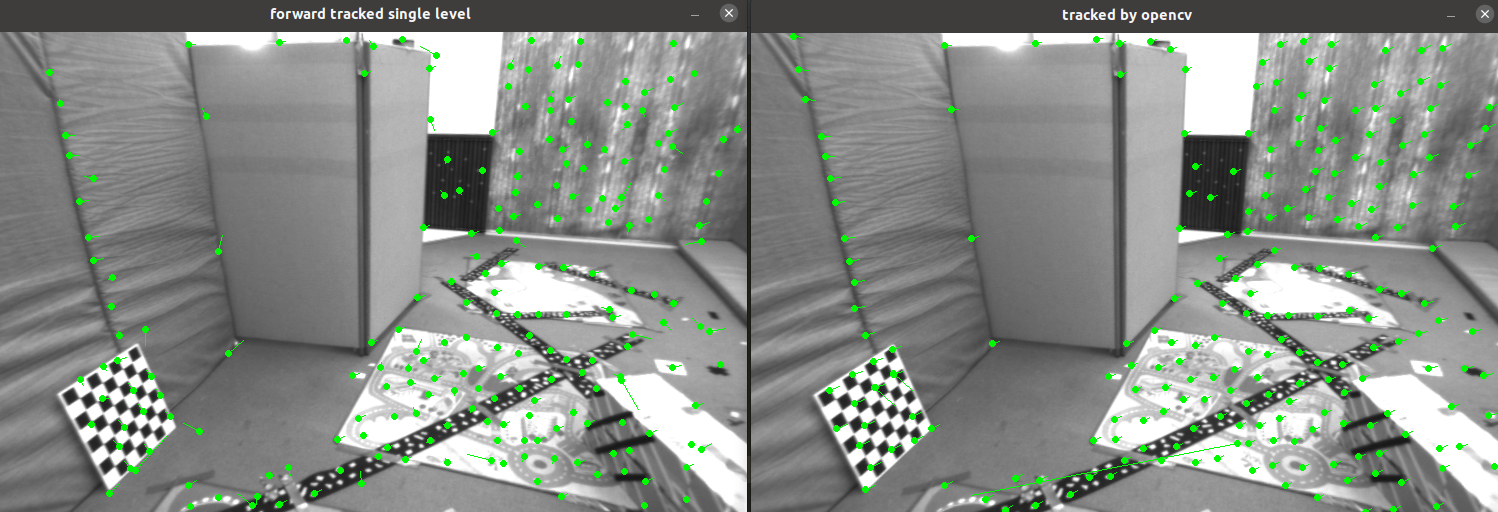
\includegraphics[width=4.8in]{ch6_2_1.png} {图2.1  前向G-N光流与OpenCV光流对比}
\end{figure}


\subsection{反向法}
反向法的光流使用$I_1$的梯度替换了$I_2$的梯度,对应的导数为:
\begin{align}
\frac{\partial I_1}{\partial x_i}=\frac{I_2(x_i+1,y_i)-I_2(x_i-1,y_i)}{2} \notag \\
\frac{\partial I_1}{\partial y_i}=\frac{I_2(x_i,y_i+1)-I_2(x_i,y_i-1)}{2}
\end{align}

代码部分见Listing1,与OpenCV的对比见图2.2,可见前向比反向法更好。
\begin{figure}[H]
\centering
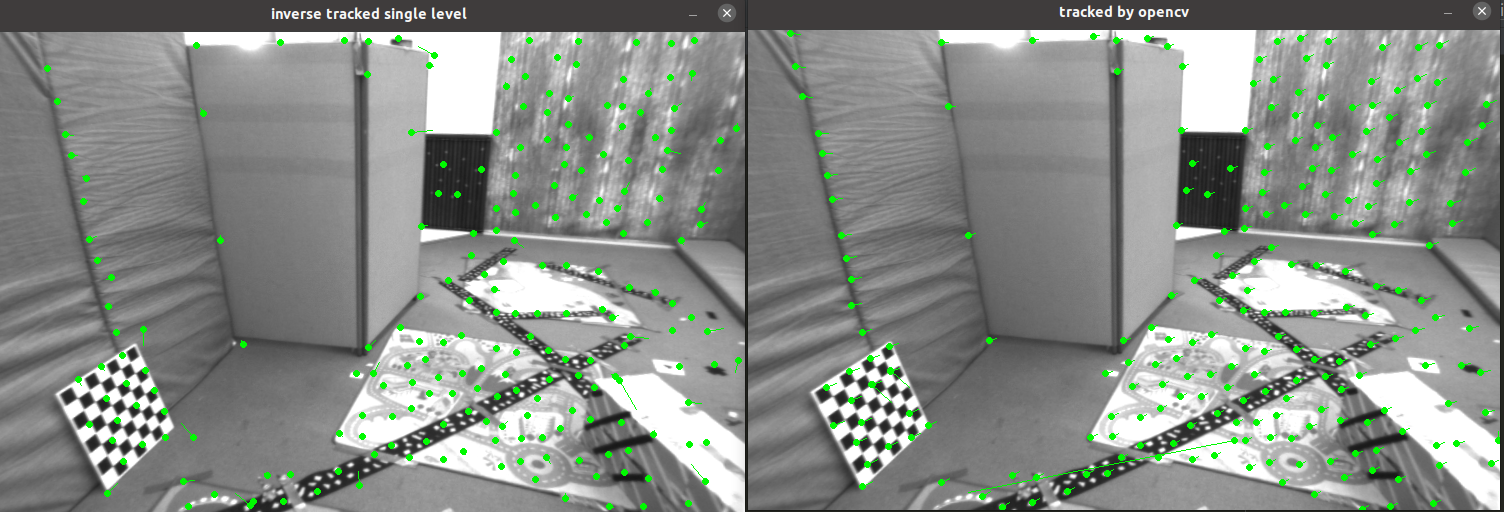
\includegraphics[width=4.8in]{ch6_2_2.png} {图2.2  反向G-N光流与OpenCV光流对比}
\end{figure}


\subsection{推广至金字塔}
\begin{enumerate}
\item 所谓 coarse-to-fine 是指怎样的过程?

如图2.3所示,左侧字底向上,以原始图像作为最底层,每往上一层,就对下一层图像进行一定倍率的缩小,得到一个金字塔;计算光流时,先将原始图像的特征点所放到左侧最顶层,然后如右侧所示,自顶向下逐层进行单层光流计算特征点,并逐层放大,本层放大后的特征点作为下层光流的初始值,自顶向下的这个过程的特征点由大到小,股也被称为由粗至精的过程(coarse to fine)。
\begin{figure}[H]
\centering
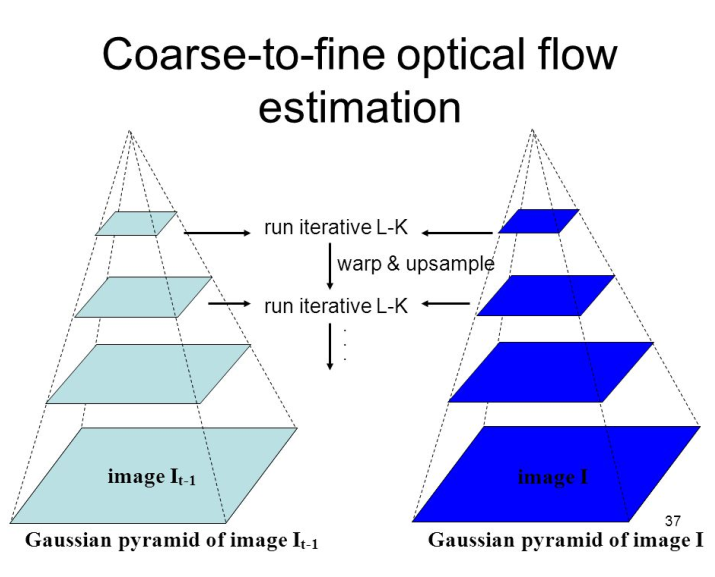
\includegraphics[scale=0.5]{ch6_2_5.png} {\\图2.3 金字塔模型}
\end{figure}

\item 光流法中的金字塔用途和特征点法中的金字塔有何差别?

光流法金字塔,可以使得优化过程更易跳出,因为光流法作为一个优化问题,必须假设优化的初始值靠近最优值,才能在一定程度上保障算法的收敛,如果相机运动较快,两张图像差异明显,单层的光流法容易达到一个局部极小值。

特征点法金字塔,其作用是解决Fast角点从远处看是角点,而进出可能不是角点的尺度问题,实现Fast角点的尺度不变性。
\end{enumerate}


金字塔代码如Listing2所示,正向和反向金字塔与OpenCV的对比如图2.4和2.5所示,可见金字塔对于正向和反向法的性能均有所提升。

\begin{lstlisting}[language=C++, caption=多层金字塔代码]
void OpticalFlowMultiLevel(
        const Mat &img1,
        const Mat &img2,
        const vector<KeyPoint> &kp1,
        vector<KeyPoint> &kp2,
        vector<bool> &success,
        bool inverse) {

    // parameters
    int pyramids = 4;  //4层金字塔
    double pyramid_scale = 0.5;  //缩放率为0.5
    double scales[] = {1.0, 0.5, 0.25, 0.125};

    // create pyramids
    vector<Mat> pyr1, pyr2; // image pyramids
    // TODO START YOUR CODE HERE (~8 lines)
    for (int i = 0; i < pyramids; i++) {
        if(i==0)
        {
            pyr1.push_back(img1);
            pyr2.push_back(img2);
        }
        else
        {
            Mat img1_pyr, img2_pyr;
            //自底向上缩放
            cv::resize(pyr1[i-1], img1_pyr, cv::Size(pyr1[i-1].cols * pyramid_scale, pyr1[i-1].rows * pyramid_scale));
            cv::resize(pyr2[i-1], img2_pyr, cv::Size(pyr2[i-1].cols * pyramid_scale, pyr2[i-1].rows * pyramid_scale));
            pyr1.push_back(img1_pyr);
            pyr2.push_back(img2_pyr);
        }
    }
    // TODO END YOUR CODE HERE

    // coarse-to-fine LK tracking in pyramids
    // TODO START YOUR CODE HERE
    vector<KeyPoint> kp1_pyr, kp2_pyr;  //特征点金字塔

//    int tmp_level = pyramids;
    for(auto &kp:kp1)
    {
        auto kp_top = kp;

        kp_top.pt *= scales[pyramids - 1];
        kp1_pyr.push_back(kp_top);
        kp2_pyr.push_back(kp_top);
    }

    for(int level = pyramids-1; level>=0; level--)
    {
        success.clear();
        OpticalFlowSingleLevel(pyr1[level], pyr2[level], kp1_pyr, kp2_pyr, success, inverse);

        if(level>0)
        {
            for(auto &kp: kp1_pyr)  //引用,改变源数据
                kp.pt /= pyramid_scale;
            for(auto &kp: kp2_pyr)
                kp.pt /= pyramid_scale;
        }
    }

    // don't forget to set the results into kp2
    for(auto &kp: kp2_pyr)
        kp2.push_back(kp);
    // TODO END YOUR CODE HERE
}
\end{lstlisting}


\begin{figure}[H]
\centering
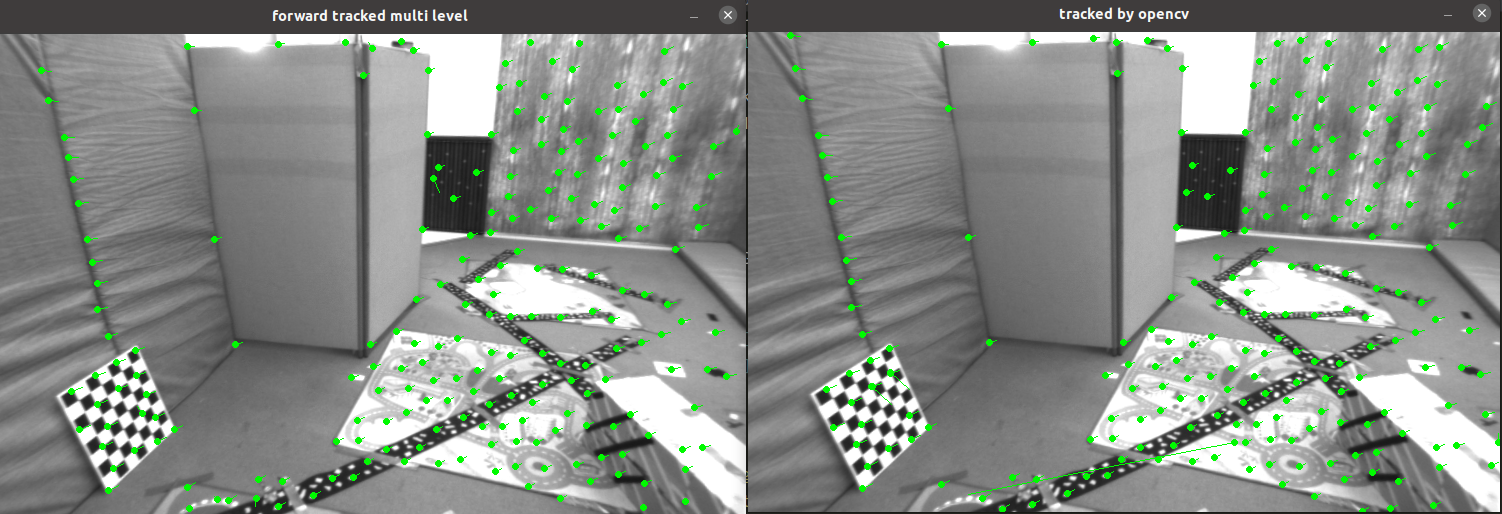
\includegraphics[width=4.8in]{ch6_2_3.png} {图2.4  正向金字塔G-N光流与OpenCV光流对比}
\end{figure}

\begin{figure}[H]
\centering
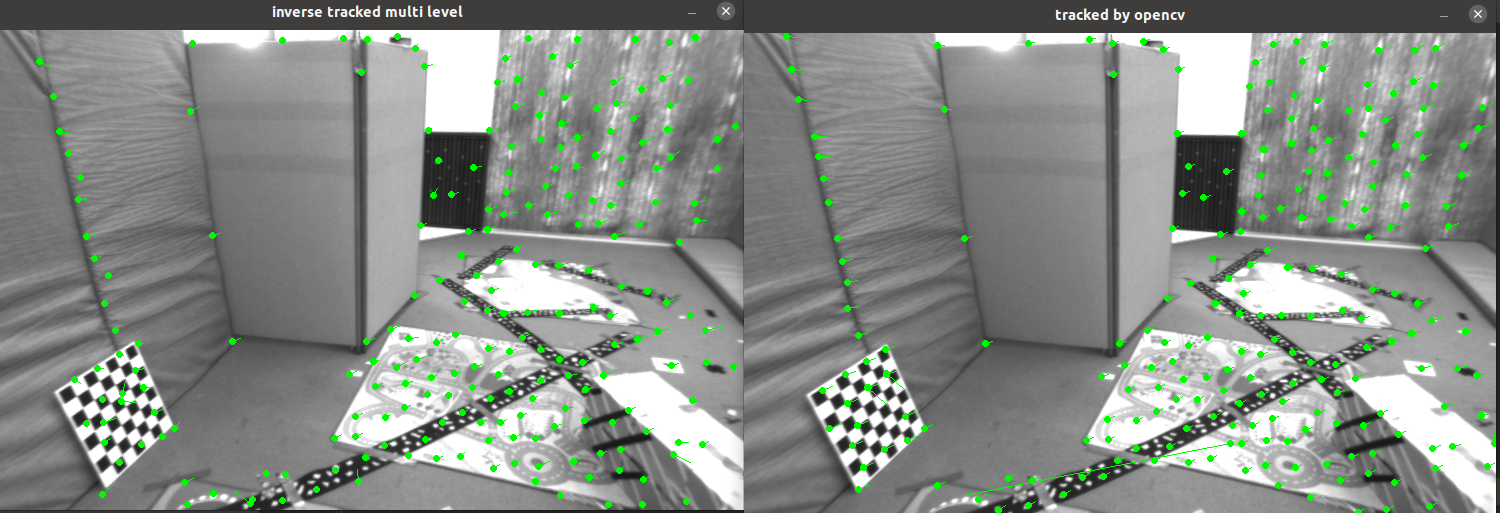
\includegraphics[width=4.8in]{ch6_2_4.png} {图2.5  反向金字塔G-N光流与OpenCV光流对比}
\end{figure}


\subsection{并行化}
引入一个额外的vector用于存放下标i,核心代码如Listing3所示。
\begin{lstlisting}[language=C++, caption=并行化核心代码]
    vector<int> indexes;
    for (int (i) = 0; (i) < kp1.size(); ++(i))
        indexes.push_back(i);
    std::mutex m;
    std::lock_guard<std::mutex> guard(m);//代替m.lock; m.unlock();
    for_each(execution::par_unseq, indexes.begin(), indexes.end(),
                  [&](auto& i)
                  {
                  //和单层光流一样
                  });
\end{lstlisting}

\begin{figure}[H]
\centering
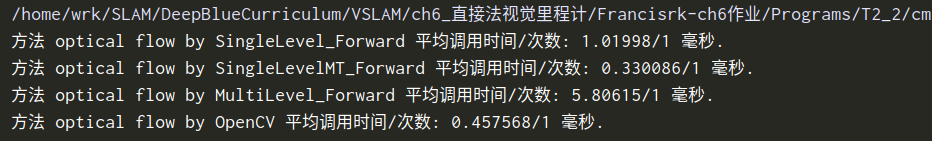
\includegraphics[width=4.8in]{ch6_2_6.png} {图2.5 并行化对比}
\end{figure}

可以看出,光流法在并行化之后速度提升0.7ms左右,有较大提升。

\subsection{讨论}
\begin{enumerate}
\item 我们优化两个图像块的灰度之差真的合理吗?哪些时候不够合理?你有解决办法吗?

优化两个图像块的灰度之差是在强假设“灰度不变假设”下进行的,即同一个空间点的像素灰度值,在各个图像中是固定不变的。当灰度不变假设成立时,这样优化合理,当物体材质变化较大、像素亮度发生剧烈变化时这样优化就不太合理。可以使用像素的相对变化来进行光流,对图像中的每个像素值减去均值,得到相对变化来做光流。还可以对像素值进行归一化。

\item 图像块大小是否有明显差异?取 16x16 和 8x8 的图像块会让结果发生变化吗?

使用OpenCV对$8\times 8$和$16\times 16$进行了对比,发现$16\times 16$的窗口效果要更好一些,$16\times 16$的基本上没有错误的方向,说明适当调整窗口大小能够优化光流追踪性能,窗口大鲁棒性好,窗口小精确性好。对比结果如图2.6所示。

\begin{figure}[H]
\centering
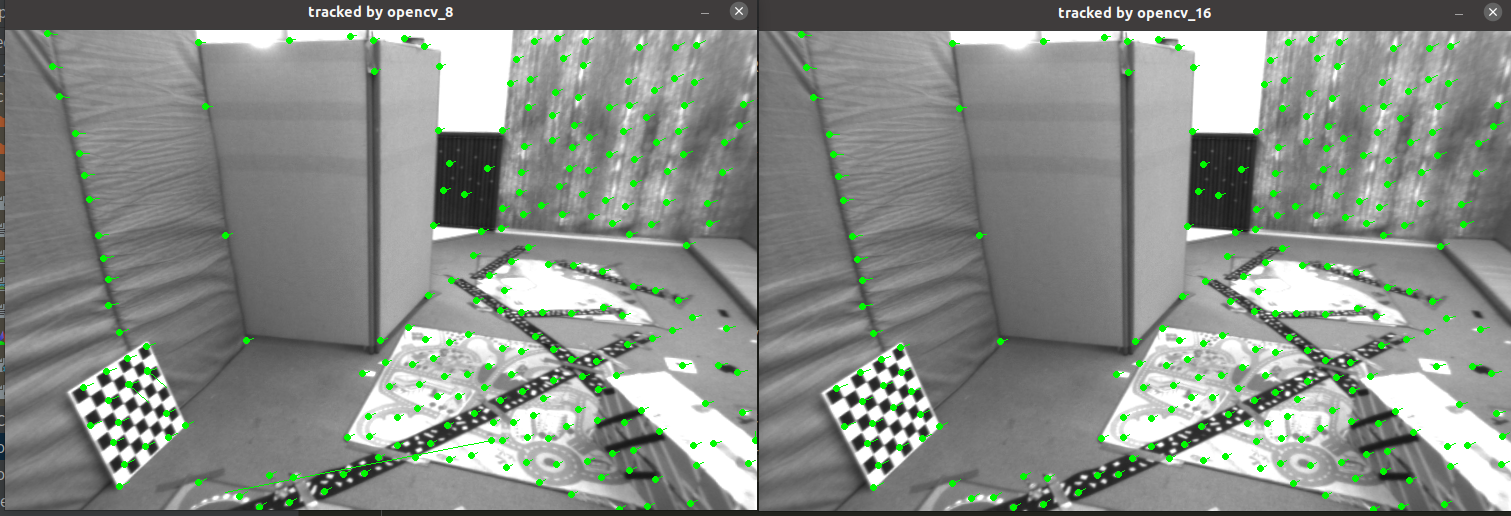
\includegraphics[width=4.8in]{ch6_2_7.png} {图2.6 $8\times 8$和$16\times 16$的窗口对比}
\end{figure}

\item 金字塔层数对结果有怎样的影响?缩放倍率呢?

金字塔层数越多,追踪的准确度越好,但是层数越多,追踪到的点就越少、越密集,边缘的点容易被忽略,越容易引起误追踪,如图2.7是3,5,7层金字塔的对比。

\begin{figure}[H]
\centering
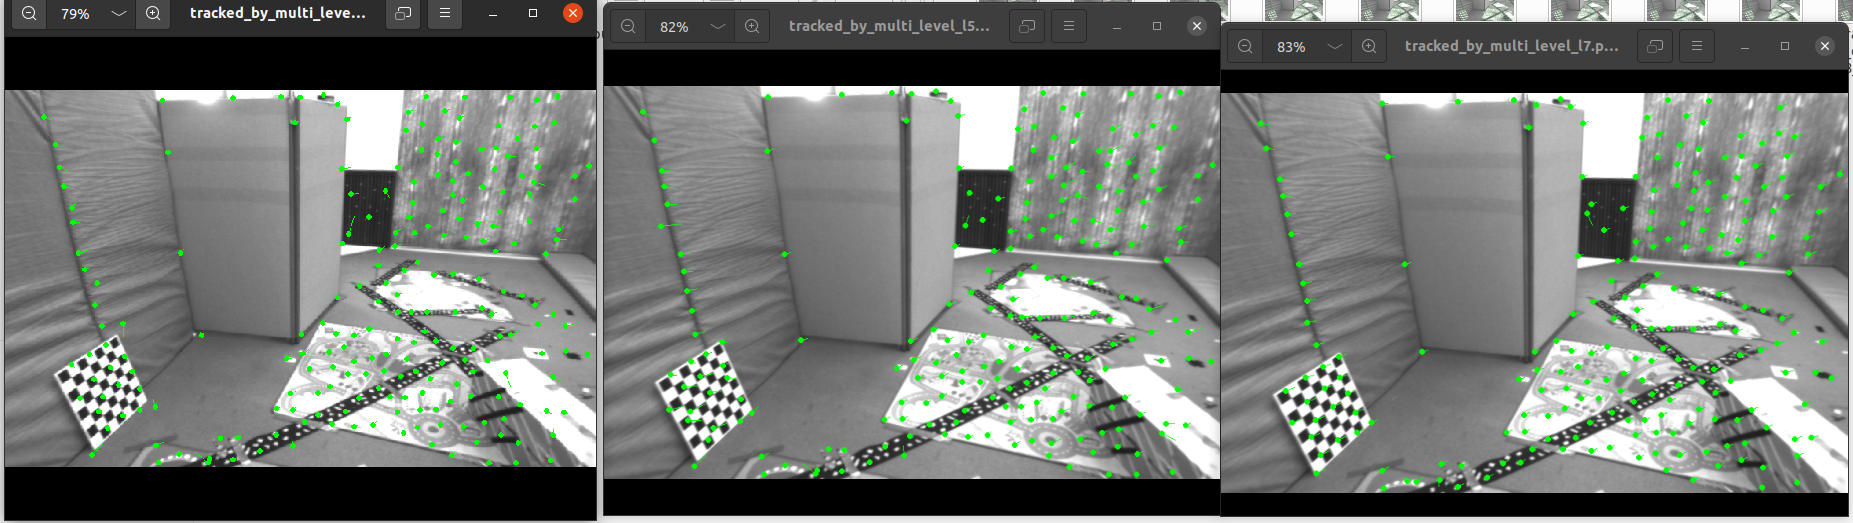
\includegraphics[width=4.8in]{ch6_2_8.png} {图2.7  3、5、7层金字塔对比}
\end{figure}


当缩放率变化时,按理来说应该变化很大(网上说倍率越小,得到的点越少,且倍率的影响比金字塔层数更大),但是经过我的实践,发现变化并不大,找了好久也没找到bug在哪里,图2.8是0.25,0.5,0.75的缩放率的对比
\begin{figure}[H]
\centering
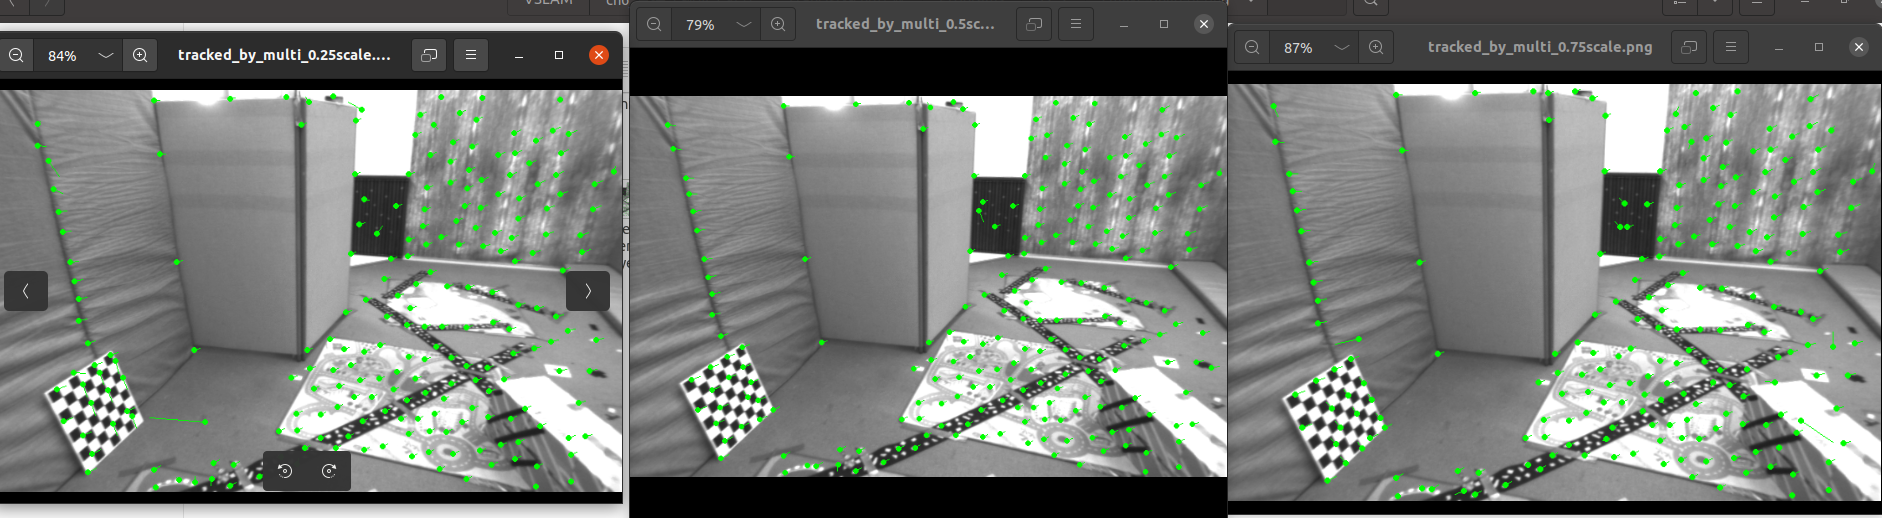
\includegraphics[width=4.8in]{ch6_2_9.png} {图2.7  0.25,0.5,0.75缩放率对比}
\end{figure}

\end{enumerate}


\section{直接法}
\subsection{单层直接法}
\begin{enumerate}
\item 该问题中的误差项是什么?

在光流法中是有特征匹配的,相当于知道了P在两张图片上的投影像素位置$P_1$,$P_2$,所以可以计算重投影的位置。而直接法事先不知道点$P_1$对应哪个点$P_2$,根据当前对相机位置的估计来寻找点$P_2$的位置,进而通过最小化两点之间的光度误差来调整相机的位姿,本题的误差为
\begin{align}
e=I_{ref}(\pi (p_i))-I_{cur}(\pi (p_i))
\end{align}

\item 误差相对于自变量的雅克比维度是多少?如何求解?

参照教材P218-220的推导,误差相对于李代数的雅可比矩阵由两部分组成:像素梯度$(\frac{\partial \bm{I_2}}{\partial \bm{u}})$和像素坐标对李代数左扰动的梯度$(\frac{\partial \bm u}{\partial \delta \bm \xi})$
前者维数为(1,2),后者为(2,6),故雅可比的维度为(1,6),关于像素梯度$\frac{\partial \bm{I_2}}{\partial \bm{u}}$,实际上这里简记为标量对行向量求导,分母的转置省略了,于是有
\begin{align}
\frac{\partial I_2}{\partial \bm{u}} &= 
\frac{\partial  I_{cur}}{\partial \bm u_i} \notag \\ 
&=
\begin{bmatrix}
\frac{\partial I_{cur}(u_i,v_i)}{\partial u_i} &
\frac{\partial I_{cur}(u_i,v_i)}{\partial v_i}
\end{bmatrix}_{1\times 2}
\end{align}
注意:(3.2)中是标量函数对行向量的求导,这里行向量的转置符号省略。

因为像素值不连续,所以使用差分代替求导,差分有前向差分、后向差分、中心差分三种,这里选择中心差分,故:
\begin{align}
\frac{\partial  I_{cur}}{\partial \bm u_i} &= 
-\frac{1}{2}
\begin{bmatrix}
I_{cur}(u+1,v)-I_{cur}(u-1,v) & I_{cur}(u,v+1)-I_{cur}(u,v-1)
\end{bmatrix}_{1\times 2}
\end{align}

对于第二部分$\frac{\partial \bm u}{\partial \delta \bm \xi}$,按照教材上的推导为
\begin{align}
\frac{\partial \bm u}{\partial \delta \bm \xi} &=
\frac{\partial \bm u_i}{\partial \delta \bm \xi} \notag \\
&=
\begin{bmatrix}
\frac{f_x}{Z} & 0 & -\frac{f_xX}{Z^2} & -\frac{f_xXY}{Z^2} & f_x+\frac{f_xX^2}{Z^2} & -\frac{f_xY}{Z} \\
0 & \frac{f_y}{Z} & -\frac{f_yY}{Z^2} & -f_y-\frac{f_yY^2}{Z^2} & \frac{f_yXY}{Z^2} & \frac{f_yX}{Z}
\end{bmatrix}_{2\times 6}
\end{align}
所以整体的雅可比矩阵为
\begin{align}
\bm J &= -\frac{\partial  I_{cur}}{\partial \bm u_i} \frac{\partial \bm u_i}{\partial \delta \bm \xi}  \notag \\
&=
-\frac{1}{2}\begin{bmatrix}
I_{cur}(u+1,v)-I_{cur}(u-1,v) & I_{cur}(u,v+1)-I_{cur}(u,v-1)
\end{bmatrix}_{1\times 2} \notag \\
& \quad *
\begin{bmatrix}
\frac{f_x}{Z} & 0 & -\frac{f_xX}{Z^2} & -\frac{f_xXY}{Z^2} & f_x+\frac{f_xX^2}{Z^2} & -\frac{f_xY}{Z} \\
0 & \frac{f_y}{Z} & -\frac{f_yY}{Z^2} & -f_y-\frac{f_yY^2}{Z^2} & \frac{f_yXY}{Z^2} & \frac{f_yX}{Z}
\end{bmatrix}_{2\times 6}
\end{align}
\end{enumerate}

核心代码如Listing4所示,对第一张图的直接法结果如图3.1所示:
\begin{lstlisting}[language=C++, caption=单层直接法核心代码]

    for (int iter = 0; iter < iterations; iter++) {
        nGood = 0;
        goodProjection.clear();

        // Define Hessian and bias
        Matrix6d H = Matrix6d::Zero();  // 6x6 Hessian
        Vector6d b = Vector6d::Zero();  // 6x1 bias

        for (size_t i = 0; i < px_ref.size(); i++)
        {

            // compute the projection in the second image
            // TODO START YOUR CODE HERE
            Eigen::Vector3d point_ref = depth_ref[i] * Eigen::Vector3d((px_ref[i][0]-cx)/fx, (px_ref[i][1]-cy)/fy, 1);  //ref中的3D点坐标
            Eigen::Vector3d point_cur = T21 * point_ref;  //ref中的3D点转换到cur中的3D点
            if (point_cur[2] < 0)   // depth invalid
                continue;

            float u = fx * point_cur[0]/point_cur[2] + cx, v = fy * point_cur[1]/point_cur[2] + cy;
            if(u<half_patch_size || u+half_patch_size>img2.cols || v<half_patch_size || v+half_patch_size>img2.rows)  //变换到cur中若越界则不优化
                continue;

            double X = point_cur[0], Y = point_cur[1], Z = point_cur[2], inv_z = 1.0 / Z, inv_z2 = inv_z * inv_z;  //cur中的3D坐标X'Y'Z'
            nGood++;
            goodProjection.push_back(Eigen::Vector2d(u, v));

            // and compute error and jacobian
            for (int x = -half_patch_size; x < half_patch_size; x++)
                for (int y = -half_patch_size; y < half_patch_size; y++)
                {
                    double error =  GetPixelValue(img1, px_ref[i][0]+x, px_ref[i][1]+y) -
                                    GetPixelValue(img2, u+x, v+y);

                    Eigen::Vector2d J_img_pixel;    // image gradients(2*1)  像素梯度,使用cur中的像素坐标和窗口偏移量x,y计算*
                    J_img_pixel<<(1.0 / 2) * (GetPixelValue(img2, u+1+x, v+y)-GetPixelValue(img2, u-1+x, v+y)),
                            (1.0 / 2) * (GetPixelValue(img2, u+x, v+1+y)-GetPixelValue(img2, u+x, v-1+y));

                    Matrix26d J_pixel_xi;   // pixel to \xi in Lie algebra  2*6
                    J_pixel_xi<<fx * inv_z,
                                0,
                                -fx * X * inv_z2,
                                -fx * X * Y * inv_z2,
                                fx + fx * X * X * inv_z2,
                                -fx * Y * inv_z,
                                0,
                                fy * inv_z,
                                -fy * Y * inv_z2,
                                -fy - fy * Y * Y * inv_z2,
                                fy * X * Y * inv_z2,
                                fy * X * inv_z;

                    // total jacobian   应该是1*6的
                    Vector6d J=-1.0 * (J_img_pixel.transpose() * J_pixel_xi).transpose();

                    H += J * J.transpose();
                    b += -error * J;
                    cost += error * error;
                }
            // END YOUR CODE HERE
        }

        // solve update and put it into estimation
        // TODO START YOUR CODE HERE
        Vector6d update = H.ldlt().solve(b);
        T21 = Sophus::SE3d::exp(update) * T21;  //李群更新
        // END YOUR CODE HERE
\end{lstlisting}

\begin{figure}[H]
\centering
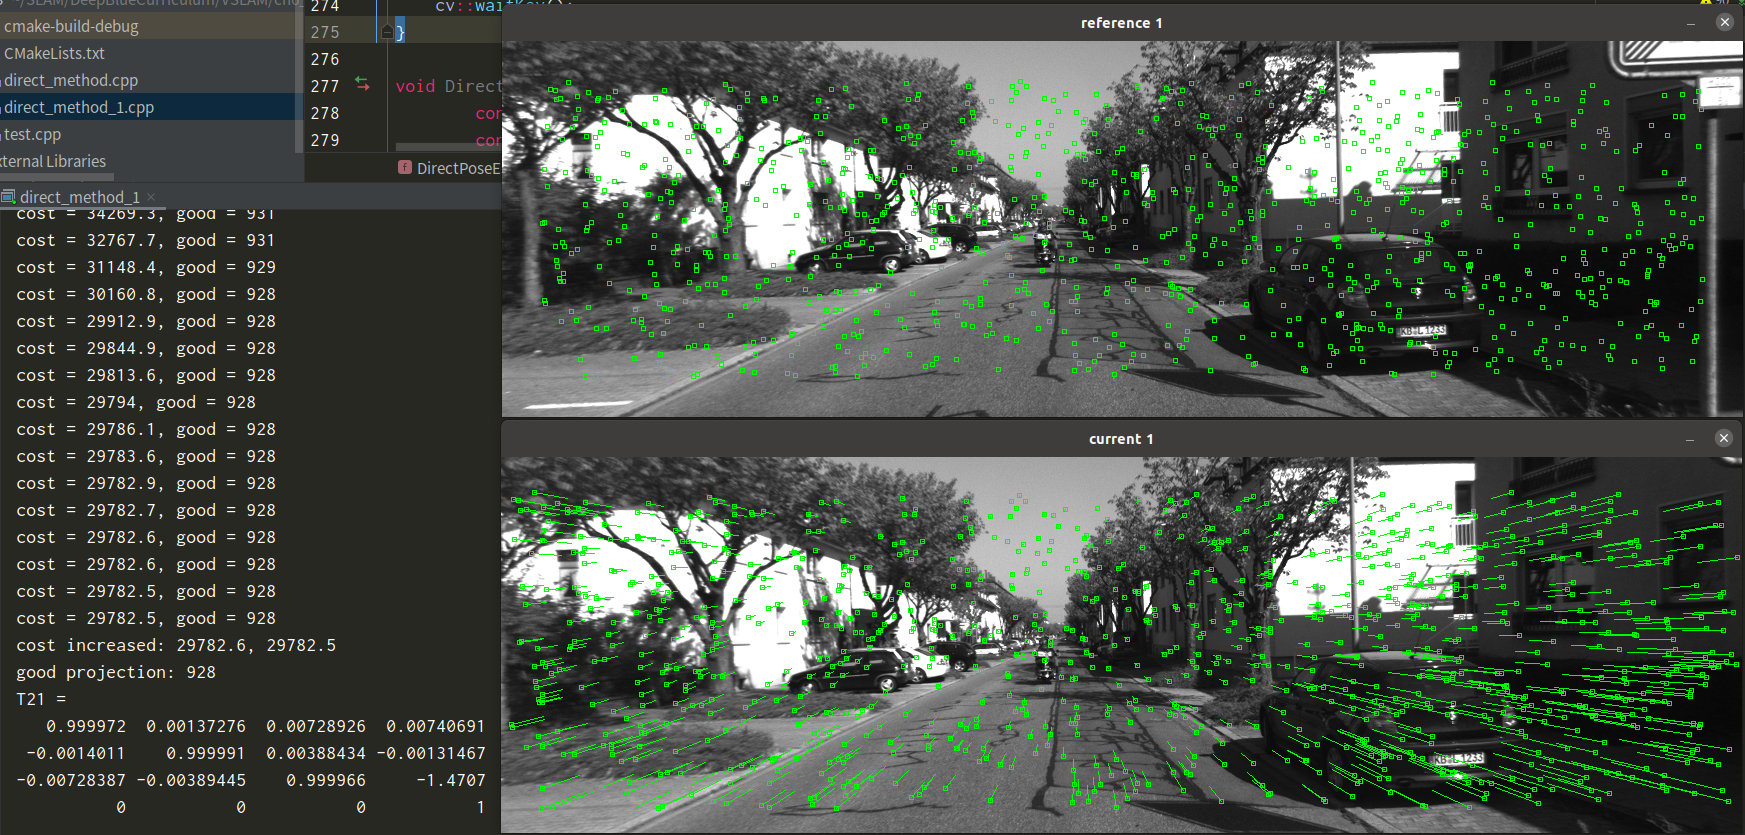
\includegraphics[width=4.8in]{ch6_3_1.png} {图3.1 单层直接法第一张图结果}
\end{figure}

\subsection{多层直接法}

\begin{enumerate}
\item 在缩放图像时,图像内参也需要跟着变化。那么,例如图像缩小一倍, fx, fy, cx, cy 应该如何变化?

相机内参也应该对应金字塔的层数做与图像对应的缩放,如Listing5所示

\begin{lstlisting}[language=C++, caption=DirectPoseEstimationMultiLayer函数]
void DirectPoseEstimationMultiLayer(
        const cv::Mat &img1,
        const cv::Mat &img2,
        const VecVector2d &px_ref,
        const vector<double> depth_ref,
        Sophus::SE3d &T21,
        string order
) {

    // parameters  4层2倍金字塔
    int pyramids = 4;
    double pyramid_scale = 0.5;
    double scales[] = {1.0, 0.5, 0.25, 0.125};

    // create pyramids
    vector<cv::Mat> pyr1, pyr2; // image pyramids
    // TODO START YOUR CODE HERE  构建图像金字塔
    for(int i=0; i<pyramids; i++)
    {
        if(i==0)
        {
            pyr1.push_back(img1);
            pyr2.push_back(img2);
        }
        else
        {
            Mat img1_pyr, img2_pyr;
            //自底向上缩放
            cv::resize(pyr1[i-1], img1_pyr, cv::Size(pyr1[i-1].cols * pyramid_scale, pyr1[i-1].rows * pyramid_scale));   //Size(width, height)
            cv::resize(pyr2[i-1], img2_pyr, cv::Size(pyr2[i-1].cols * pyramid_scale, pyr2[i-1].rows * pyramid_scale));
            pyr1.push_back(img1_pyr);
            pyr2.push_back(img2_pyr);
        }
    }

    // END YOUR CODE HERE
    //构建特征点金字塔
    double fxG = fx, fyG = fy, cxG = cx, cyG = cy;  // backup the old values
    for (int level = pyramids - 1; level >= 0; level--) {
        VecVector2d px_ref_pyr; // set the keypoints in this pyramid level
        for (auto &px: px_ref) {
            px_ref_pyr.push_back(scales[level] * px);
        }

        // TODO START YOUR CODE HERE
        // scale fx, fy, cx, cy in different pyramid levels
        fx = fxG * scales[level];
        fy = fyG * scales[level];
        cx = cxG * scales[level];
        cy = cyG * scales[level];
        // END YOUR CODE HERE
        DirectPoseEstimationSingleLayer(pyr1[level], pyr2[level], px_ref_pyr, depth_ref, T21, order);
    }
}
\end{lstlisting}
\end{enumerate}

第5张图的结果如图3.6所示



\begin{figure}[H]
\centering
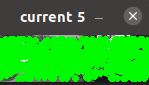
\includegraphics[scale=1]{ch6_3_4.png} {\\图3.2 多层直接法,图5第1层}
\end{figure}

\begin{figure}[H]
\centering
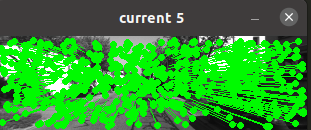
\includegraphics[scale=1]{ch6_3_5.png} {\\图3.3 多层直接法,图5第2层}
\end{figure}

\begin{figure}[H]
\centering
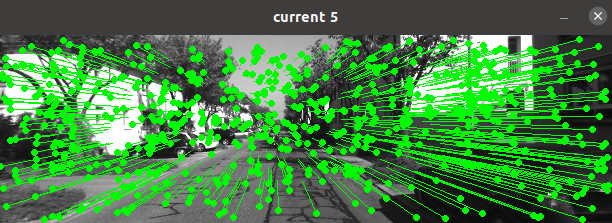
\includegraphics[scale=0.8]{ch6_3_6.png} {\\图3.4 多层直接法,图5第3层}
\end{figure}

\begin{figure}[H]
\centering
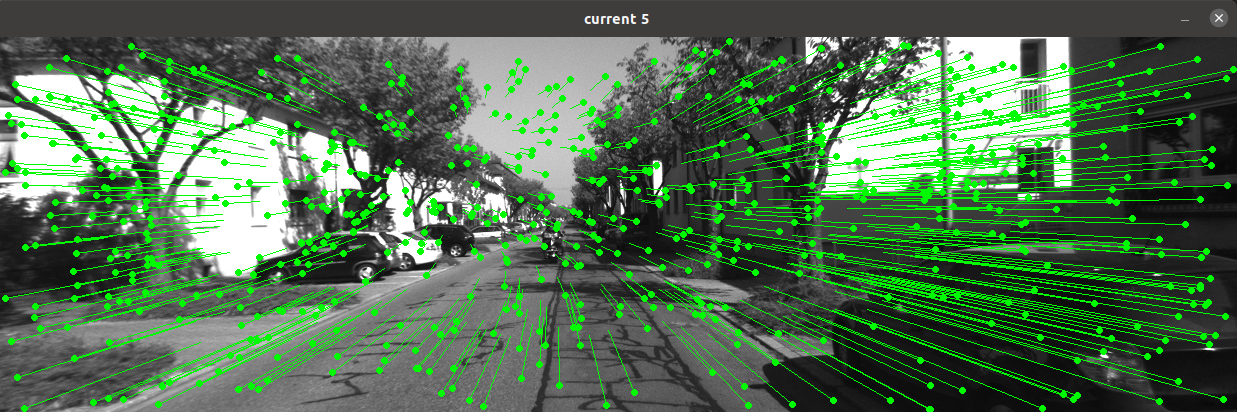
\includegraphics[scale=0.45]{ch6_3_2.png} {\\图3.5 多层直接法,图5第4层}
\end{figure}

\begin{figure}[H]
\centering
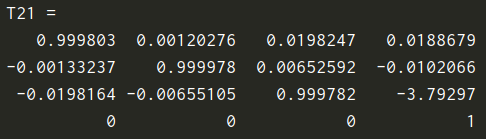
\includegraphics[width=4.8in]{ch6_3_3.png} {图3.6 估计结果}
\end{figure}

\subsection{并行化}
使用for\_each和execution进行改进,在遍历ref中的特征点处使用多线程并发,注意在对有序容器进行插入前需要加锁,核心代码如下:

\begin{lstlisting}[language=C++, caption=DirectPoseEstimationMultiLayer函数]
        // Define Hessian and bias
        Matrix6d H = Matrix6d::Zero();  // 6x6 Hessian
        Vector6d b = Vector6d::Zero();  // 6x1 bias

        vector<int> ref_index;
        for(int i=0;i<px_ref.size();++i)
            ref_index.push_back(i);

        std::mutex m;
        for_each(execution::par_unseq, ref_index.begin(), ref_index.end(),
                 [&](auto& i)
                 {
                     // compute the projection in the second image
                     // TODO START YOUR CODE HERE
                     Eigen::Vector3d point_ref = depth_ref[i] * Eigen::Vector3d((px_ref[i][0]-cx)/fx, (px_ref[i][1]-cy)/fy, 1);  //ref中的3D点坐标
                     Eigen::Vector3d point_cur = T21 * point_ref;  //ref中的3D点转换到cur中的3D点
                     if (point_cur[2] >= 0)   // depth invalid
                     {
                         float u = fx * point_cur[0]/point_cur[2] + cx, v = fy * point_cur[1]/point_cur[2] + cy;
                         if(u>=half_patch_size && u+half_patch_size<=img2.cols && v>=half_patch_size && v+half_patch_size<=img2.rows)  //变换到cur中若越界则不优化
                         {
                             double X = point_cur[0], Y = point_cur[1], Z = point_cur[2], inv_z = 1.0 / Z, inv_z2 = inv_z * inv_z;  //cur中的3D坐标X'Y'Z'
                             nGood++;
                             std::lock_guard<std::mutex> guard(m);//代替m.lock; m.unlock();
                             //记录投影前后的uv坐标
                             goodProjection.push_back(Eigen::Vector2d(u, v));
                             GoodRefIndex.push_back(Eigen::Vector2d(px_ref[i][0],px_ref[i][1]));
\end{lstlisting}

选择两张000001.png和000002.png分别与单进程进行对比,普通单层和并行化单层运行时间比较如图3.7-3.8所示
\begin{figure}[H]
\centering
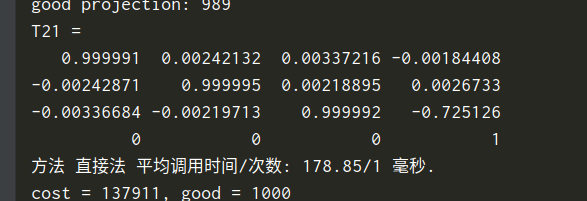
\includegraphics[width=4.8in]{ch6_3_8_1.png} 
\end{figure}

\begin{figure}[H]
\centering
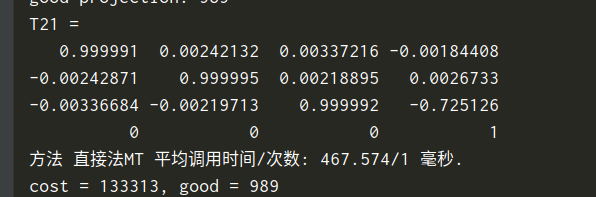
\includegraphics[width=4.8in]{ch6_3_8_2.png} {图3.7 估计结果\_1}
\end{figure}

\begin{figure}[H]
\centering
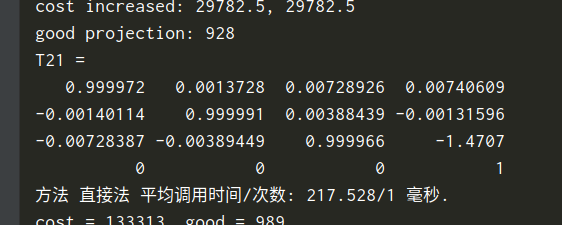
\includegraphics[width=4.8in]{ch6_3_8_3.png} 
\end{figure}

\begin{figure}[H]
\centering
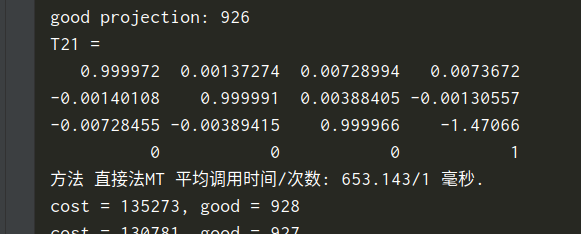
\includegraphics[width=4.8in]{ch6_3_8_4.png} {图3.8 估计结果\_2}
\end{figure}

可以看出,并行化之后速度略微有些变慢,具体是什么原因呢?

\subsection{延伸讨论}
\begin{enumerate}
\item 直接法是否可以类似光流,提出 inverse, compositional 的概念?它们有意义吗?

可以提出inverse,compositional的概念,但是没有意义。因为,直接法必须计算两张图片整体的光度误差,而不是估计图像中像素的相对运动。

\item 请思考上面算法哪些地方可以缓存或加速?

在遍历每个选择的特征点时可以使用并行加速遍历。另外,窗口的大小可以适当调整,不是越大越好,窗口越大计算量越大,速度越慢。

\item 在上述过程中,我们实际假设了哪两个 patch 不变?

1.灰度值不变(同一空间点在各个视角下成像的灰度不变) \\
2.同一窗口内的深度信息不变\\
如下列代码所示:
\begin{lstlisting}[language=C++]
double error =  GetPixelValue(img1, px_ref[i][0]+x, px_ref[i][1]+y) - GetPixelValue(img2, u+x, v+y);
\end{lstlisting}

\item 为何可以随机取点?而不用取角点或线上的点?那些不是角点的地方,投影算对了吗?

因为直接法对计算光度误差进行优化,雅可比表示当像素梯度不为0即对优化有贡献,所以不是角点的地方,只要保证有像素梯度即可。

\item 请总结直接法相对于特征点法的异同与优缺点。

优点: \\
1.可以省去计算特征点、描述子的时间。

2.只要求有像素梯度即可,不需要特征点。

3.可以构建半稠密乃至稠密的地图,这点是特征点无法做到的。

缺点:

1.非凸性。

2.单个像素没有区分度。

3.灰度值不变是很强的假设。
具体在十四讲第二版P230-231。
\end{enumerate}


\section{使用光流计算视差} 
使用LK光流计算left中的GFTT特征点在right中的对应,根据坐标的对应关系计算出水平视差,计算视差的核心代码如Listing7所示,计算结果如图4.1所示,OpenCV的光流法之后的视差平均误差为-24.5884。
\begin{lstlisting}[language=C++, caption=计算视差的核心代码]
    //OpenCV
    Mat img2_CV;
    cv::cvtColor(img2, img2_CV, CV_GRAY2BGR);
    for (int i = 0; i < pt2.size(); i++) {
        if (status[i]) {
            cv::circle(img2_CV, pt2[i], 2, cv::Scalar(0, 250, 0), 2);
            cv::line(img2_CV, pt1[i], pt2[i], cv::Scalar(0, 250, 0));
            dis = kp1[i].pt.x - kp2_single[i].pt.x;
            cost.push_back(dis- GetPixelValue(disparity_img, kp1[i].pt.x, kp1[i].pt.y));
        }
    }
    cost_sum = accumulate(cost.begin(), cost.end(), 0.0);  //求和
    cout<<"OpenCV光流平均误差:"<<cost_sum/cost.size()<<endl;
    cost.clear();
\end{lstlisting}

\begin{figure}[H]
\centering
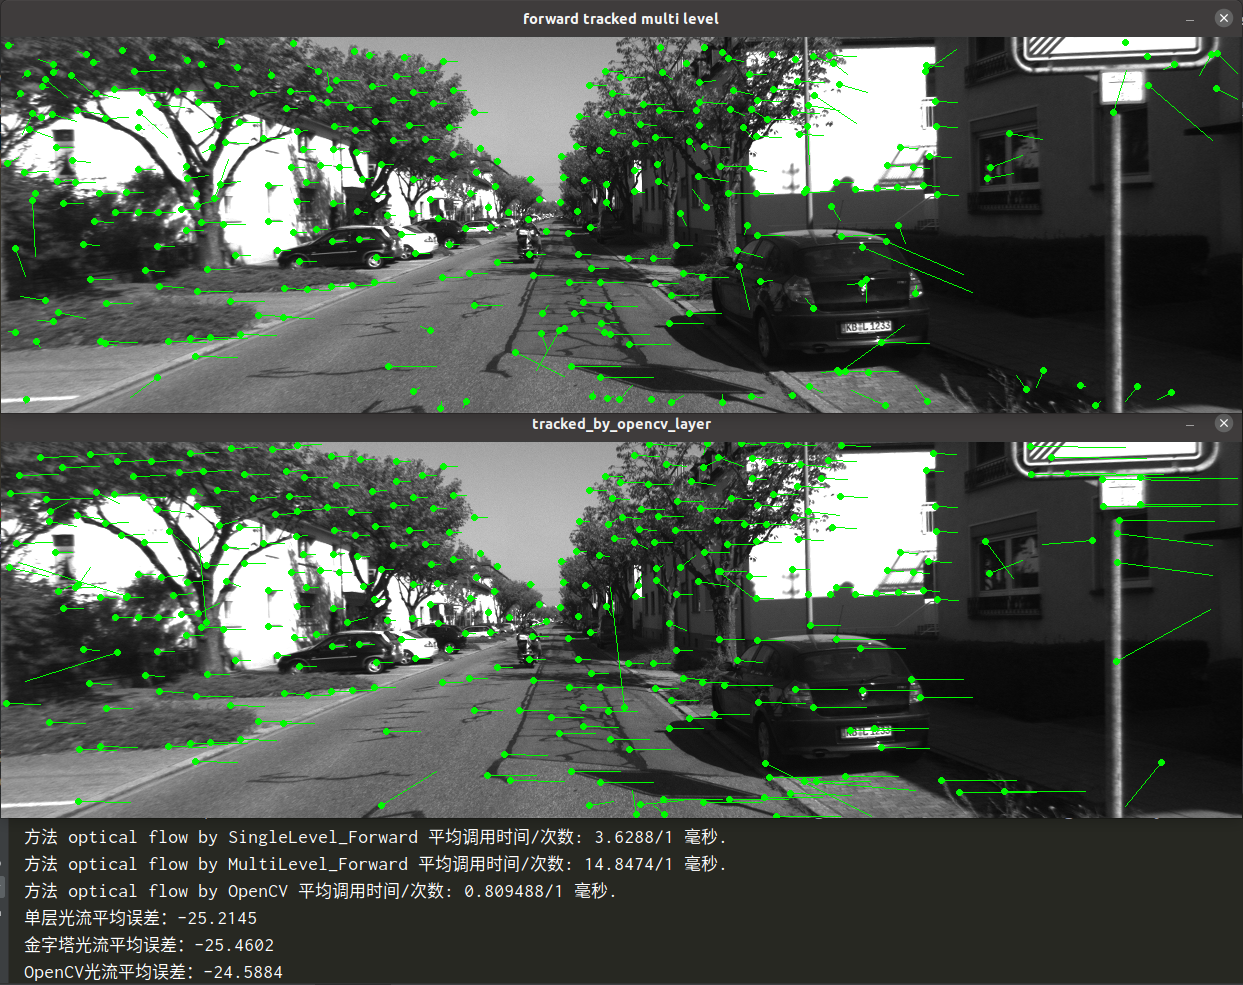
\includegraphics[width=4.8in]{ch6_4_1.png} {图4.1 视差计算结果}
\end{figure}



\begin{thebibliography}{99}  
\bibitem{ref1}https://zhuanlan.zhihu.com/p/101092663
\bibitem{ref2}https://blog.csdn.net/jiachang98/article/details/121269827?spm=1001.2014.3001.5502
\end{thebibliography}




\end{document}